%Unrolling a graph to a tree, equivalent to message passing. Identifying loops.
%DRNN paper claims TreeLSTM can't be used for decoding. Sure it can.

%More general recursive neural networks and structures that work beyond RNNs are  
%rarer. Seq2Tree, Tree2Seq, Tree2Tree, Graphs
%Trees reduce "long-term"ness (and functional decomposition)

%Only pass in a bottom-up encoding?

% Generating graphs with cycles/message-passing?

%Variable misuse, assuming all variables exist and don't need to be declared.

%Semantic encoding -> syntactic decoding
		
%Decoding can use progressively less information.

%Encoding and decoding can even go in different directions

%Try to have an enncoding that doesn't contain any other bugs.

%Encoding:  all the leaves have different outputs. Hmmm...

%The encoder basically becomes the decoder if trained to just predict `next''
%token generatively. If not, we need to pass all possible nodes to the decoder 
%as ``starting points''.

%If two nodes share the same decomposition, then the model can't distinguish 
%them.

%We move topology prediction to be before the node generation?

%for (int i = 0; i < 10; i++) {
%	printf("%d\n", i);
%}

\section{Introduction}\label{sec:introduction}

Traditionally, tasks in program analysis treated source code as a linear 
sequence of tokens.  Without any further modeling, a recurrent neural network 
(RNN) trained on such sequences is theoretically able to learn the underlying 
dependencies---the \textit{structure}---of the sequence elements.  The structure 
is implicit in the parameters of the RNN and in the values of the hidden states.
\begin{figure}[ht]
\begin{center}
	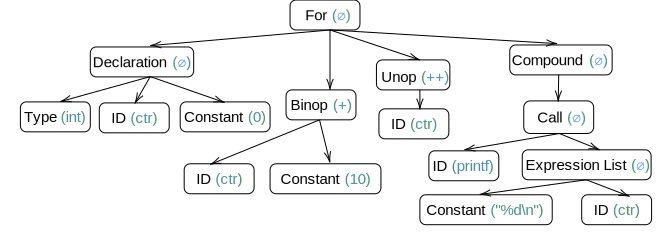
\includegraphics[width=\textwidth]{figures/ast.png}
\end{center}
\caption{An example abstract syntax tree for the C programming 
language.}\label{fig:ast}
\end{figure}



However, while source code may be linear, its execution is fundamentally 
nonlinear. A sequential model trained on source code has to learn these 
nonlinearities, often without any actual sense of a language's semantics.  A 
program's abstract syntax tree (AST), as seen in Figure~\ref{fig:ast}, is one 
step closer to modeling the nonlinearity in a program. Recent work has placed 
increasing emphasis on \textit{explicitly} modeling the underlying structure of 
such nonlinear data (see Section~\ref{sec:related}).


%By explicitly working on parse trees for natural language tasks and abstract 
%syntax trees (ASTs) for program analysis tasks, we simplify the learning task
%Even BERT, though linear, removes the directionality bias inherenet in RNNs.  
%What benefits?  Nonlinearity.  Limits on the ability for the RNN to memorize


To this end, we introduce the notion of \textit{relational decomposition}, with 
which one can readily express complicated dependencies between elements in 
structured data. At a high level, relational decomposition involves applying 
prior knowledge to break down structured data into smaller chunks that are 
individually easier to learn, and then aggregating the results from all chunks. 

For example, if we know in advance that a particular node in a tree only depends 
on its immediate ancestors, then we can narrow the focus of the learning task to 
just that relational path through the tree. In decomposing a problem, we find 
that being able to use relational operators directly is invaluable, such as 
using composition to specify ``siblings of my parent''. Given these operators, 
we find that many mechanisms such as attention are readily expressed in 
relational terms, even without applying relational decomposition.



%Relational decomposition provides a natural way of modeling trees as 
%combinations of relationships. For example, doubly-recurrent neural networks 
%(DRNNs)\cite{alvarez2016tree} decompose nodes into parent paths and 
%left-sibling paths (see Figure~\ref{fig:broken}).
%In the case of DRNNs, the relative paths form sequences that can be trained with 
%two independent RNNs. However, an individual relation may be modeled with 
%feed-forward neural network, bidirectional RNNs, graph neural networks, or even 
%a non-deep-learning module.

%A further challenge in modeling source code is arbitrary identifiers. In 
%section, we demonstrate how relational decomposition over ASTs simplifies this 
%task.
%
%Although we use ASTs as motivating examples throughout the paper, relational 
%decomposition readily applies to other structured tasks. 


%Applications of machine learning to programming offer great promise: bug 
%detection, automatic program repair, program synthesis, code understanding, 
%autocompletion, variable name suggestion, program translation, program 
%analysis, automated test generation, and so on.  However, two properties of 
%source code present recurring difficulty to modern algorithms: arbitrary 
%user-defined identifiers and nonlinearity.  Arbitrary identifiers mean that two 
%variables with the same purpose may not share a name, and also neural networks 
%have a finite dictionary. We return to the point of arbitrary identifiers later 
%in the paper, for now focusing on nonlinearity.


% int ctr = 0;
% for (int i = 0; i < 10; i++)
% for (int j = 0; j < 10; j++)
% for (int k = 0; k < 10; k++)
% ctr += 1; return 10;

%" These results suggest that it is the
%need to integrate structures far apart in the sentence that characterizes the tasks where recursive
%models surpass recurrent models."
% \cite{DBLP:journals/corr/LiJH15}
% Also, outputs are much more likely to compile/be syntactically valid

%In recent years, increasing effort has focused on using the inherent structure 
%of source code.  In doing so, we can improve training speed and learnability.  
%However, In general, this requires learning the relationship between 
%\textit{all} variables in the input and output.  Attempt to model the structure 
%directly.  Inductive bias
%
%The simplest example of a structure is a sequence, for which RNNs (and LSTMs) 
%have thrived.  They have transformed speech recognition, language translation, 
%etc.

\begin{figure}[ht]\label{fig:preorder}
\begin{center}


\tikzset{every picture/.style={line width=0.75pt}} %set default line width to 0.75pt        

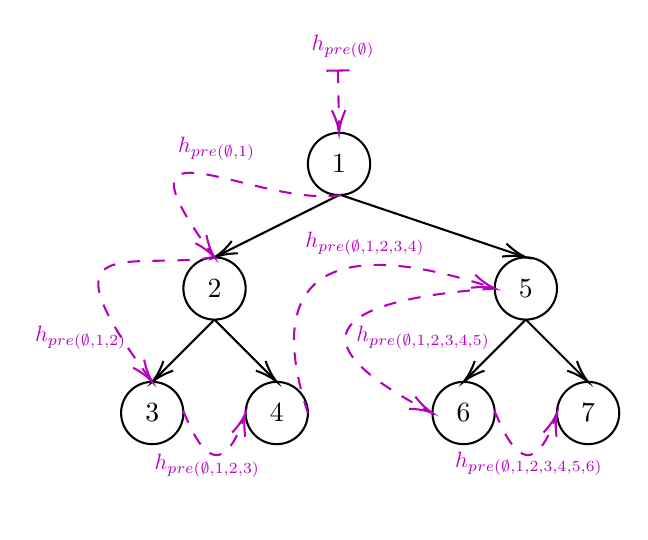
\begin{tikzpicture}[x=0.75pt,y=0.75pt,yscale=-1,xscale=1]
%uncomment if require: \path (0,247.3125); %set diagram left start at 0, and has height of 247.3125

%Shape: Circle [id:dp5747539528933221] 
\draw   (150,75) .. controls (150,66.72) and (156.72,60) .. (165,60) .. controls (173.28,60) and (180,66.72) .. (180,75) .. controls (180,83.28) and (173.28,90) .. (165,90) .. controls (156.72,90) and (150,83.28) .. (150,75) -- cycle ;
%Shape: Circle [id:dp6584741963271383] 
\draw   (90,135) .. controls (90,126.72) and (96.72,120) .. (105,120) .. controls (113.28,120) and (120,126.72) .. (120,135) .. controls (120,143.28) and (113.28,150) .. (105,150) .. controls (96.72,150) and (90,143.28) .. (90,135) -- cycle ;
%Shape: Circle [id:dp42608384351679063] 
\draw   (240,135) .. controls (240,126.72) and (246.72,120) .. (255,120) .. controls (263.28,120) and (270,126.72) .. (270,135) .. controls (270,143.28) and (263.28,150) .. (255,150) .. controls (246.72,150) and (240,143.28) .. (240,135) -- cycle ;
%Shape: Circle [id:dp4039562507165959] 
\draw   (60,195) .. controls (60,186.72) and (66.72,180) .. (75,180) .. controls (83.28,180) and (90,186.72) .. (90,195) .. controls (90,203.28) and (83.28,210) .. (75,210) .. controls (66.72,210) and (60,203.28) .. (60,195) -- cycle ;
%Shape: Circle [id:dp6061665496522999] 
\draw   (120,195) .. controls (120,186.72) and (126.72,180) .. (135,180) .. controls (143.28,180) and (150,186.72) .. (150,195) .. controls (150,203.28) and (143.28,210) .. (135,210) .. controls (126.72,210) and (120,203.28) .. (120,195) -- cycle ;
%Straight Lines [id:da040054788995673274] 
\draw    (165,90) -- (106.79,119.11) ;
\draw [shift={(105,120)}, rotate = 333.43] [color={rgb, 255:red, 0; green, 0; blue, 0 }  ][line width=0.75]    (10.93,-3.29) .. controls (6.95,-1.4) and (3.31,-0.3) .. (0,0) .. controls (3.31,0.3) and (6.95,1.4) .. (10.93,3.29)   ;

%Straight Lines [id:da9417356343431731] 
\draw    (166,90) -- (253.1,119.36) ;
\draw [shift={(255,120)}, rotate = 198.63] [color={rgb, 255:red, 0; green, 0; blue, 0 }  ][line width=0.75]    (10.93,-3.29) .. controls (6.95,-1.4) and (3.31,-0.3) .. (0,0) .. controls (3.31,0.3) and (6.95,1.4) .. (10.93,3.29)   ;

%Straight Lines [id:da7471003825026084] 
\draw    (105,150) -- (76.41,178.59) ;
\draw [shift={(75,180)}, rotate = 315] [color={rgb, 255:red, 0; green, 0; blue, 0 }  ][line width=0.75]    (10.93,-3.29) .. controls (6.95,-1.4) and (3.31,-0.3) .. (0,0) .. controls (3.31,0.3) and (6.95,1.4) .. (10.93,3.29)   ;

%Straight Lines [id:da3919517743443004] 
\draw    (105,150) -- (133.59,178.59) ;
\draw [shift={(135,180)}, rotate = 225] [color={rgb, 255:red, 0; green, 0; blue, 0 }  ][line width=0.75]    (10.93,-3.29) .. controls (6.95,-1.4) and (3.31,-0.3) .. (0,0) .. controls (3.31,0.3) and (6.95,1.4) .. (10.93,3.29)   ;

%Shape: Circle [id:dp09204588637656741] 
\draw   (210,195) .. controls (210,186.72) and (216.72,180) .. (225,180) .. controls (233.28,180) and (240,186.72) .. (240,195) .. controls (240,203.28) and (233.28,210) .. (225,210) .. controls (216.72,210) and (210,203.28) .. (210,195) -- cycle ;
%Shape: Circle [id:dp4405799901518632] 
\draw   (270,195) .. controls (270,186.72) and (276.72,180) .. (285,180) .. controls (293.28,180) and (300,186.72) .. (300,195) .. controls (300,203.28) and (293.28,210) .. (285,210) .. controls (276.72,210) and (270,203.28) .. (270,195) -- cycle ;
%Straight Lines [id:da9350681939269714] 
\draw    (255,150) -- (226.41,178.59) ;
\draw [shift={(225,180)}, rotate = 315] [color={rgb, 255:red, 0; green, 0; blue, 0 }  ][line width=0.75]    (10.93,-3.29) .. controls (6.95,-1.4) and (3.31,-0.3) .. (0,0) .. controls (3.31,0.3) and (6.95,1.4) .. (10.93,3.29)   ;

%Straight Lines [id:da6947341181570368] 
\draw    (255,150) -- (283.59,178.59) ;
\draw [shift={(285,180)}, rotate = 225] [color={rgb, 255:red, 0; green, 0; blue, 0 }  ][line width=0.75]    (10.93,-3.29) .. controls (6.95,-1.4) and (3.31,-0.3) .. (0,0) .. controls (3.31,0.3) and (6.95,1.4) .. (10.93,3.29)   ;

%Curve Lines [id:da39887266209810046] 
\draw [color={rgb, 255:red, 182; green, 0; blue, 192 }  ,draw opacity=1 ] [dash pattern={on 4.5pt off 4.5pt}]  (166,90) .. controls (124.21,96.28) and (50.74,46.81) .. (104.18,118.9) ;
\draw [shift={(105,120)}, rotate = 233.26] [color={rgb, 255:red, 182; green, 0; blue, 192 }  ,draw opacity=1 ][line width=0.75]    (10.93,-3.29) .. controls (6.95,-1.4) and (3.31,-0.3) .. (0,0) .. controls (3.31,0.3) and (6.95,1.4) .. (10.93,3.29)   ;

%Curve Lines [id:da20716783829208452] 
\draw [color={rgb, 255:red, 182; green, 0; blue, 192 }  ,draw opacity=1 ] [dash pattern={on 4.5pt off 4.5pt}]  (105,120) .. controls (63.21,126.28) and (20.43,106.51) .. (74.18,178.9) ;
\draw [shift={(75,180)}, rotate = 233.26] [color={rgb, 255:red, 182; green, 0; blue, 192 }  ,draw opacity=1 ][line width=0.75]    (10.93,-3.29) .. controls (6.95,-1.4) and (3.31,-0.3) .. (0,0) .. controls (3.31,0.3) and (6.95,1.4) .. (10.93,3.29)   ;

%Curve Lines [id:da03343755971007978] 
\draw [color={rgb, 255:red, 182; green, 0; blue, 192 }  ,draw opacity=1 ] [dash pattern={on 4.5pt off 4.5pt}]  (150,195) .. controls (124.63,117.7) and (174.99,113.35) .. (239.03,134.68) ;
\draw [shift={(240,135)}, rotate = 198.57999999999998] [color={rgb, 255:red, 182; green, 0; blue, 192 }  ,draw opacity=1 ][line width=0.75]    (10.93,-3.29) .. controls (6.95,-1.4) and (3.31,-0.3) .. (0,0) .. controls (3.31,0.3) and (6.95,1.4) .. (10.93,3.29)   ;

%Curve Lines [id:da25925997339396334] 
\draw [color={rgb, 255:red, 182; green, 0; blue, 192 }  ,draw opacity=1 ] [dash pattern={on 4.5pt off 4.5pt}]  (240,135) .. controls (177.81,139.29) and (130.97,154.16) .. (208.82,194.39) ;
\draw [shift={(210,195)}, rotate = 207.1] [color={rgb, 255:red, 182; green, 0; blue, 192 }  ,draw opacity=1 ][line width=0.75]    (10.93,-3.29) .. controls (6.95,-1.4) and (3.31,-0.3) .. (0,0) .. controls (3.31,0.3) and (6.95,1.4) .. (10.93,3.29)   ;

%Curve Lines [id:da04019975701917122] 
\draw [color={rgb, 255:red, 182; green, 0; blue, 192 }  ,draw opacity=1 ] [dash pattern={on 4.5pt off 4.5pt}]  (240,195) .. controls (239.51,189.37) and (254.2,242.24) .. (269.54,196.42) ;
\draw [shift={(270,195)}, rotate = 467.79] [color={rgb, 255:red, 182; green, 0; blue, 192 }  ,draw opacity=1 ][line width=0.75]    (10.93,-3.29) .. controls (6.95,-1.4) and (3.31,-0.3) .. (0,0) .. controls (3.31,0.3) and (6.95,1.4) .. (10.93,3.29)   ;

%Straight Lines [id:da47300784385513417] 
\draw [color={rgb, 255:red, 182; green, 0; blue, 192 }  ,draw opacity=1 ] [dash pattern={on 4.5pt off 4.5pt}]  (164.5,30) -- (164.97,58) ;
\draw [shift={(165,60)}, rotate = 269.05] [color={rgb, 255:red, 182; green, 0; blue, 192 }  ,draw opacity=1 ][line width=0.75]    (10.93,-3.29) .. controls (6.95,-1.4) and (3.31,-0.3) .. (0,0) .. controls (3.31,0.3) and (6.95,1.4) .. (10.93,3.29)   ;
\draw [shift={(164.5,30)}, rotate = 269.05] [color={rgb, 255:red, 182; green, 0; blue, 192 }  ,draw opacity=1 ][line width=0.75]    (0,5.59) -- (0,-5.59)   ;
%Curve Lines [id:da4854965313512276] 
\draw [color={rgb, 255:red, 182; green, 0; blue, 192 }  ,draw opacity=1 ] [dash pattern={on 4.5pt off 4.5pt}]  (90,195) .. controls (89.51,189.37) and (104.2,242.24) .. (119.54,196.42) ;
\draw [shift={(120,195)}, rotate = 467.79] [color={rgb, 255:red, 182; green, 0; blue, 192 }  ,draw opacity=1 ][line width=0.75]    (10.93,-3.29) .. controls (6.95,-1.4) and (3.31,-0.3) .. (0,0) .. controls (3.31,0.3) and (6.95,1.4) .. (10.93,3.29)   ;


% Text Node
\draw (165,75) node  [align=left] {1};
% Text Node
\draw (105,135) node  [align=left] {2};
% Text Node
\draw (255,135) node  [align=left] {5};
% Text Node
\draw (120,138) node  [align=left] {$ $};
% Text Node
\draw (75,195) node  [align=left] {3};
% Text Node
\draw (135,195) node  [align=left] {4};
% Text Node
\draw (225,195) node  [align=left] {6};
% Text Node
\draw (285,195) node  [align=left] {7};
% Text Node
\draw (167,18.5) node [scale=0.8,color={rgb, 255:red, 182; green, 0; blue, 192 }  ,opacity=1 ] [align=left] {$\displaystyle h_{pre( \emptyset )}$};
% Text Node
\draw (106,67.5) node [scale=0.8,color={rgb, 255:red, 182; green, 0; blue, 192 }  ,opacity=1 ] [align=left] {$\displaystyle h_{pre( \emptyset ,1)}$};
% Text Node
\draw (40.5,158.5) node [scale=0.8,color={rgb, 255:red, 182; green, 0; blue, 192 }  ,opacity=1 ] [align=left] {$\displaystyle h_{pre( \emptyset ,1,2)}$};
% Text Node
\draw (101.5,220.5) node [scale=0.8,color={rgb, 255:red, 182; green, 0; blue, 192 }  ,opacity=1 ] [align=left] {$\displaystyle h_{pre( \emptyset ,1,2,3)}$};
% Text Node
\draw (177.5,113.5) node [scale=0.8,color={rgb, 255:red, 182; green, 0; blue, 192 }  ,opacity=1 ] [align=left] {$\displaystyle h_{pre( \emptyset ,1,2,3,4)}$};
% Text Node
\draw (205.5,158.5) node [scale=0.8,color={rgb, 255:red, 182; green, 0; blue, 192 }  ,opacity=1 ] [align=left] {$\displaystyle h_{pre( \emptyset ,1,2,3,4,5)}$};
% Text Node
\draw (256.5,219.5) node [scale=0.8,color={rgb, 255:red, 182; green, 0; blue, 192 }  ,opacity=1 ] [align=left] {$\displaystyle h_{pre( \emptyset ,1,2,3,4,5,6)}$};


\end{tikzpicture}

\end{center}
\caption{Preorder}
\end{figure}

\input{figures/left_subtree}
\begin{figure}[ht]\label{fig:cell}
\begin{center}



\tikzset{every picture/.style={line width=0.75pt}} %set default line width to 0.75pt        

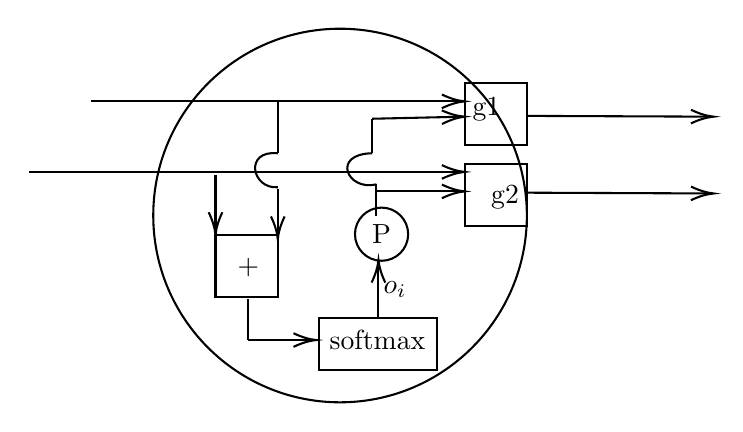
\begin{tikzpicture}[x=0.75pt,y=0.75pt,yscale=-1,xscale=1]
%uncomment if require: \path (0,247.3125); %set diagram left start at 0, and has height of 247.3125

%Shape: Circle [id:dp6083722186206264] 
\draw   (300,90) .. controls (300,40.29) and (340.29,0) .. (390,0) .. controls (439.71,0) and (480,40.29) .. (480,90) .. controls (480,139.71) and (439.71,180) .. (390,180) .. controls (340.29,180) and (300,139.71) .. (300,90) -- cycle ;
%Straight Lines [id:da561245922461306] 
\draw    (270,35) -- (448,35) ;
\draw [shift={(450,35)}, rotate = 180] [color={rgb, 255:red, 0; green, 0; blue, 0 }  ][line width=0.75]    (10.93,-3.29) .. controls (6.95,-1.4) and (3.31,-0.3) .. (0,0) .. controls (3.31,0.3) and (6.95,1.4) .. (10.93,3.29)   ;

%Straight Lines [id:da18790606634377727] 
\draw    (240,69) -- (448,69) ;
\draw [shift={(450,69)}, rotate = 180] [color={rgb, 255:red, 0; green, 0; blue, 0 }  ][line width=0.75]    (10.93,-3.29) .. controls (6.95,-1.4) and (3.31,-0.3) .. (0,0) .. controls (3.31,0.3) and (6.95,1.4) .. (10.93,3.29)   ;

%Shape: Square [id:dp2745914981980191] 
\draw   (450,26) -- (480,26) -- (480,56) -- (450,56) -- cycle ;
%Shape: Square [id:dp4400376186234609] 
\draw   (450,65) -- (480,65) -- (480,95) -- (450,95) -- cycle ;
%Shape: Square [id:dp5494449586600998] 
\draw   (330,99.38) -- (360,99.38) -- (360,129.38) -- (330,129.38) -- cycle ;
%Straight Lines [id:da5818908117859822] 
\draw    (345.5,150) -- (376.5,150) ;
\draw [shift={(378.5,150)}, rotate = 180] [color={rgb, 255:red, 0; green, 0; blue, 0 }  ][line width=0.75]    (10.93,-3.29) .. controls (6.95,-1.4) and (3.31,-0.3) .. (0,0) .. controls (3.31,0.3) and (6.95,1.4) .. (10.93,3.29)   ;

%Shape: Rectangle [id:dp8507803775022897] 
\draw   (380,139.38) -- (436.5,139.38) -- (436.5,164.38) -- (380,164.38) -- cycle ;
%Straight Lines [id:da5079909504409219] 
\draw    (408.5,139.38) -- (408.5,113.38) ;
\draw [shift={(408.5,111.38)}, rotate = 450] [color={rgb, 255:red, 0; green, 0; blue, 0 }  ][line width=0.75]    (10.93,-3.29) .. controls (6.95,-1.4) and (3.31,-0.3) .. (0,0) .. controls (3.31,0.3) and (6.95,1.4) .. (10.93,3.29)   ;

%Straight Lines [id:da24915260067311573] 
\draw    (330,70.38) -- (330,97.38) ;
\draw [shift={(330,99.38)}, rotate = 270] [color={rgb, 255:red, 0; green, 0; blue, 0 }  ][line width=0.75]    (10.93,-3.29) .. controls (6.95,-1.4) and (3.31,-0.3) .. (0,0) .. controls (3.31,0.3) and (6.95,1.4) .. (10.93,3.29)   ;

%Straight Lines [id:da08640126621337885] 
\draw    (360,35) -- (360,60) ;


%Straight Lines [id:da7146155948789545] 
\draw    (360,77.38) -- (360,99.38) ;
\draw [shift={(360,101.38)}, rotate = 270] [color={rgb, 255:red, 0; green, 0; blue, 0 }  ][line width=0.75]    (10.93,-3.29) .. controls (6.95,-1.4) and (3.31,-0.3) .. (0,0) .. controls (3.31,0.3) and (6.95,1.4) .. (10.93,3.29)   ;

%Curve Lines [id:da3867366642345542] 
\draw    (360,76.38) .. controls (347.5,77.38) and (343.5,58.38) .. (360,60) ;


%Straight Lines [id:da5452257068640174] 
\draw    (345.5,130.38) -- (345.5,150) ;


%Straight Lines [id:da40110507885008895] 
\draw    (407.5,75) -- (407.5,90) ;


%Curve Lines [id:da38530851203182825] 
\draw    (407.5,75) .. controls (393.5,78.38) and (385.5,60.38) .. (405.5,60) ;


%Straight Lines [id:da4735381882476042] 
\draw    (405.5,43.38) -- (448,42.42) ;
\draw [shift={(450,42.38)}, rotate = 538.71] [color={rgb, 255:red, 0; green, 0; blue, 0 }  ][line width=0.75]    (10.93,-3.29) .. controls (6.95,-1.4) and (3.31,-0.3) .. (0,0) .. controls (3.31,0.3) and (6.95,1.4) .. (10.93,3.29)   ;

%Straight Lines [id:da9357133547762917] 
\draw    (405.5,43.38) -- (405.5,60) ;


%Straight Lines [id:da9994096101128709] 
\draw    (407.5,78.38) -- (448,78.38) ;
\draw [shift={(450,78.38)}, rotate = 180] [color={rgb, 255:red, 0; green, 0; blue, 0 }  ][line width=0.75]    (10.93,-3.29) .. controls (6.95,-1.4) and (3.31,-0.3) .. (0,0) .. controls (3.31,0.3) and (6.95,1.4) .. (10.93,3.29)   ;

%Straight Lines [id:da6130989952789851] 
\draw    (480,42) -- (568,42.37) ;
\draw [shift={(570,42.38)}, rotate = 180.24] [color={rgb, 255:red, 0; green, 0; blue, 0 }  ][line width=0.75]    (10.93,-3.29) .. controls (6.95,-1.4) and (3.31,-0.3) .. (0,0) .. controls (3.31,0.3) and (6.95,1.4) .. (10.93,3.29)   ;

%Straight Lines [id:da28139602174802314] 
\draw    (480,79) -- (568,79.37) ;
\draw [shift={(570,79.38)}, rotate = 180.24] [color={rgb, 255:red, 0; green, 0; blue, 0 }  ][line width=0.75]    (10.93,-3.29) .. controls (6.95,-1.4) and (3.31,-0.3) .. (0,0) .. controls (3.31,0.3) and (6.95,1.4) .. (10.93,3.29)   ;


% Text Node
\draw (345.81,115.19) node  [align=left] {+};
% Text Node
\draw (408,150) node  [align=left] {softmax};
% Text Node
\draw (416.5,125.5) node  [align=left] {$\displaystyle o_{i}$};
% Text Node
\draw    (410, 99) circle [x radius= 12.81, y radius= 12.81]   ;
\draw (410,99) node  [align=left] {P};
% Text Node
\draw (460.5,39) node  [align=left] {g1};
% Text Node
\draw (469.5,81) node  [align=left] {g2};


\end{tikzpicture}


\end{center}
\caption{Cell}
\end{figure}



%Relational decomposition not just as a way of reasoning, but programming.

%\item Step back for encoding, decoding, attention, even residual connections.
The major contribution of this work is the introduction of the relational 
decomposition framework. To this end, we:

\begin{itemize}
% TODO: decomposition over nodes?
\item formalize the notion of relational decomposition, including an analysis of 
relational operators decompositions over trees.

\item reframe standard attention mechanisms as a form of higher-order relation.  
	With this framing, we identify \textit{relative attention} as a natural 
	generalization of attention over relations.
	We further apply relative attention to construct a novel relational form of 
	pointer networks.

\item concretize relational decomposition as a \textit{framework} by providing a 
library written in Python and Tensorflow that simplifies the task of relational 
reasoning.

%The library, called {\tt Trooper}, is available at XYZ.
%Tensorflow library allowing for higher-level reasoning over structured data.

\item cast prior work within the relational decomposition framework.
	%In particular, doubly-recurrent neural networks (DRNNs) are a simple 
	%decomposition of trees.  However, we identify a flaw that severely limits the 
	%applicability of DRNNs to abstract syntax trees, and suggest natural 
	%extensions to the decomposition that overcome these limitations.

Extensibility
Modularity
Reproducability
Translation to other tasks (we can easily apply it to anything that can feed us 
a graph of the right form).

\item Evaluate relationally-motivated extensions of prior models.
\end{itemize}

%Doubly-recurrent neural networks (DRNNs)\cite{alvarez2016tree} are a specific 
%instance, where the two relations are just the left-sibling and parent. 
%However, take the example in Figure~\ref{fig:broken}. We are generating the 
%tree top-down, left-to-right. We have made it all the way to generating node D.
%
